
\chapter{Methodology}\label{chap:related_works}


\section{Configuration}\label{sec:2-spec}
In this experimental setup, two fundamental sensors are employed to acquire and analyze data.
The Realsense D435i camera, 
known for its high-resolution image capture and depth-sensing capabilities, is utilized for visual data acquisition. 
Complementing the camera is the AWR1843boost mmWave radar, operating in the 77-81GHz frequency range. 
Both sensors are securely housed within a custom 3D-printed enclosure, 
which not only safeguards them but also minimizes external interference, ensuring the integrity of data acquisition. 
The mmWave radar config that is used is a 77-81GHz chirp, with settings balanced between range and resolution,
collecting data at 20 frames per second.

\begin{figure}[hpbt]
    \centering
    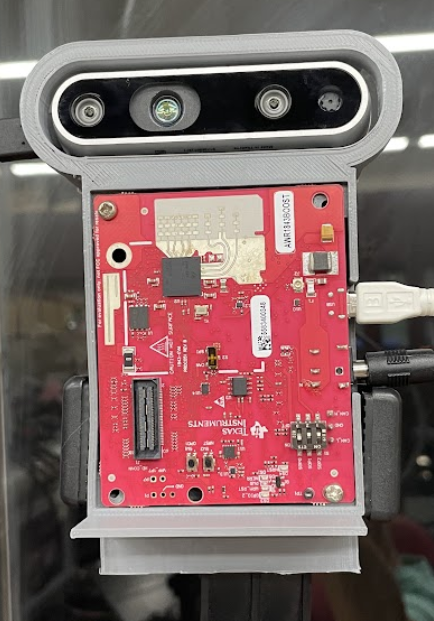
\includegraphics[width=10cm]{Figures/radar_camera_setup.png}%\textwidth
    \caption{Radar camera setup}
    \label{fig:radar_camera_setup_fig}
\end{figure}


\section{Overview}\label{sec:2-overview}
Overview block diagram of the project  
\begin{figure}[hpbt]
    \centering
    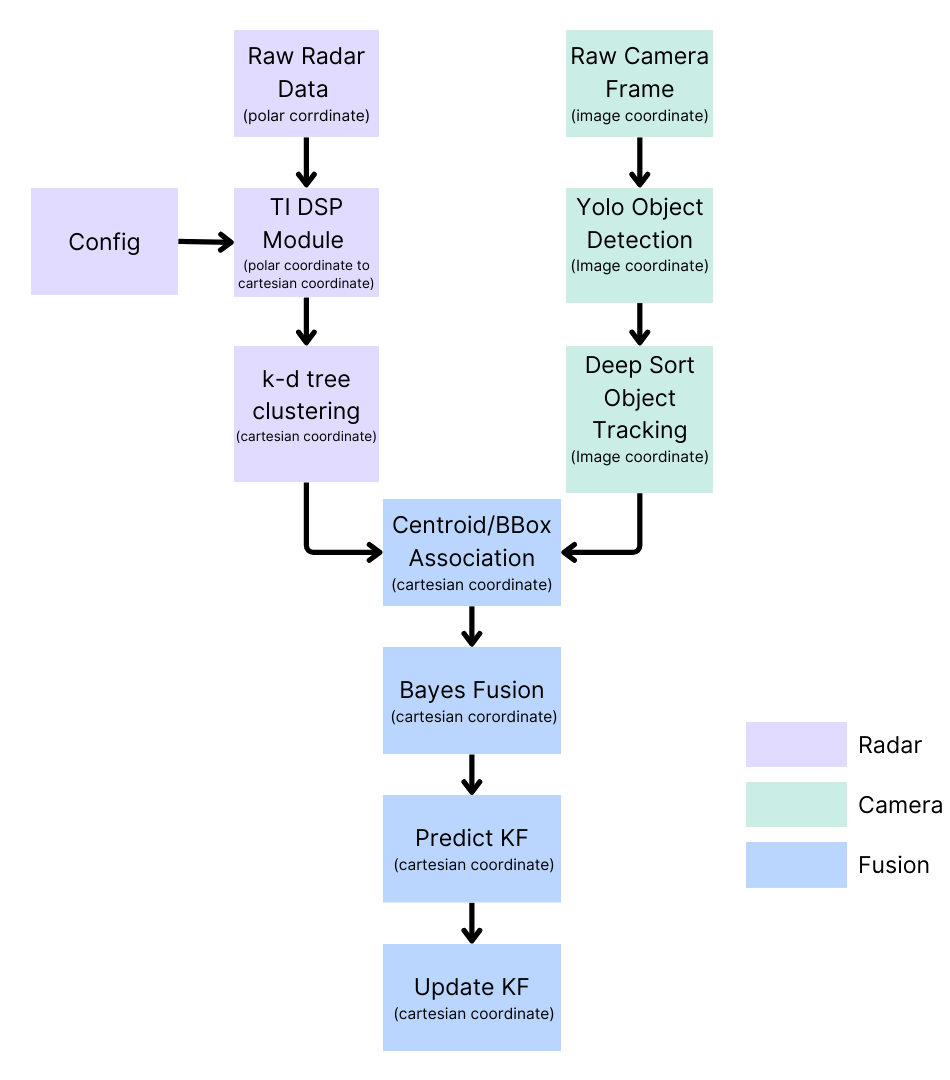
\includegraphics[width=12cm]{Figures/kf_update-modified.png}%\textwidth
    \caption{Radar camera Kalman Filter workflow}
    \label{fig:kf_update}
\end{figure}

\section{Calibration}\label{sec:2-calibration}
\subsection{Camera Calibration}
To accurately map the monocular camera's image coordinates to real-world coordinates, calibration of intrinsic and extrinsic is required.
Using tools provided by ROS \cite{cam_calib}.

\begin{figure}[hpbt]
    \centering
    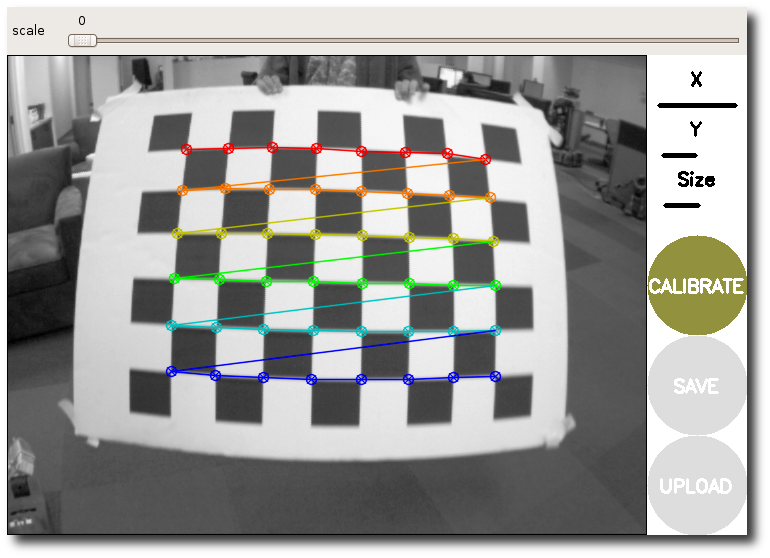
\includegraphics[width=8cm]{Figures/cam_calib.png}%\textwidth
    \caption{Camera extrinsic and intrinsic calibration}
    \label{fig:camera_calibration}
\end{figure}

\subsection{Radar-Camera Calibration}
In order to achieve accurate sensor fusion, it is essential to conduct proper calibration of the two sensors. 
For this purpose, a corner reflector is employed, primarily due to its strong radar reflection characteristics. 
Additionally, it offers the advantage of appearing as a single point in both radar and camera data, effectively reducing ambiguity.

As illustrated in Figure <insert figure>, data points from both radar 
and camera coordinates can be collected with the corner reflector positioned at various locations.
\begin{figure}[hbpt]
    \centering
    \begin{subfigure}{0.25\linewidth}
        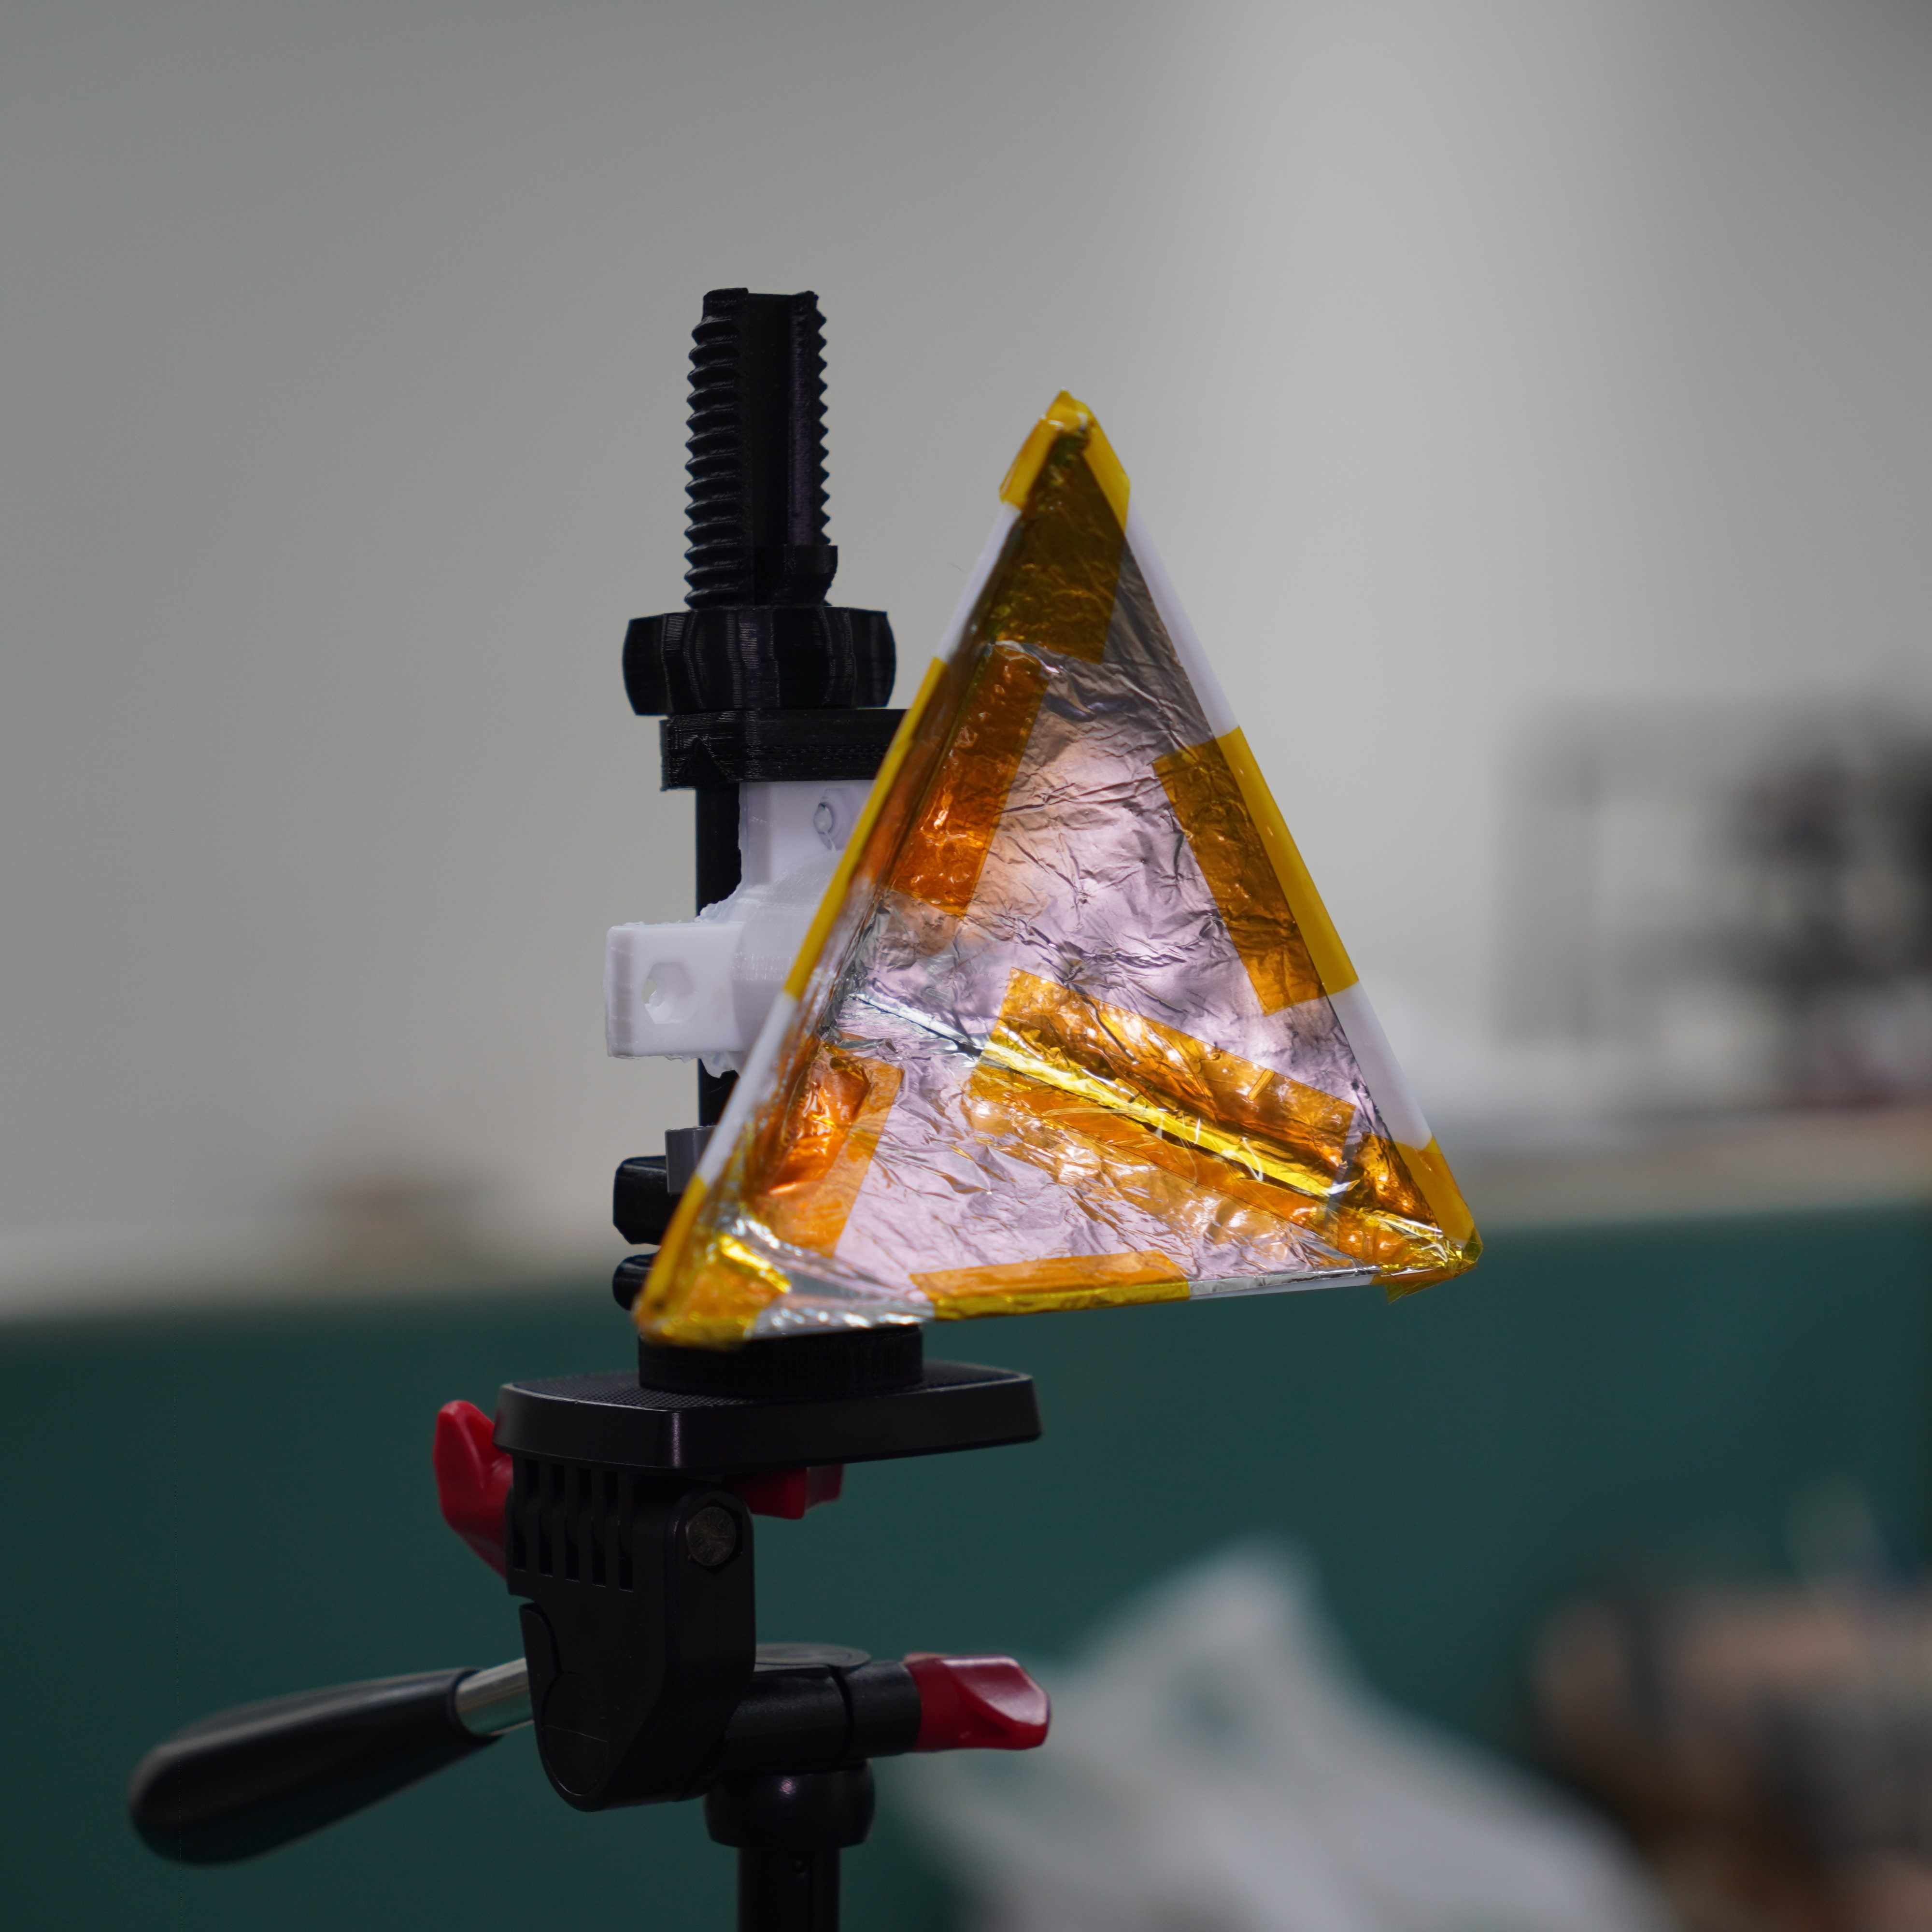
\includegraphics[width=5.5cm]{Figures/corner_reflector.jpg}
        \caption{Radar Corner Reflector}
    \end{subfigure}
    \hfill
    \begin{subfigure}{0.25\linewidth}
        \centering
        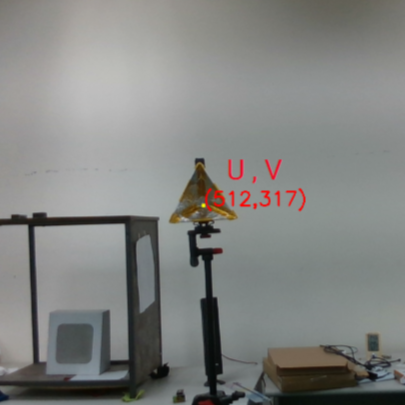
\includegraphics[width=5.5cm]{Figures/camera_corner.png}
        \caption{Camera-corner reflector calibration}
    \end{subfigure}
    \hfill
    \begin{subfigure}{0.25\linewidth}
        \centering
        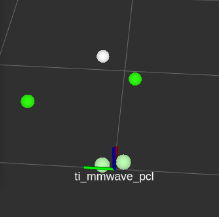
\includegraphics[width=5.5cm]{Figures/radar_corner.png}
        \caption{Radar-corner reflector calibration}
    \end{subfigure}

    \caption{Radar camera calibration}
    \label{fig:radar_camera_calibration}
\end{figure}

\section{Data Pre-Processing}\label{sec:2-preprocessing}
\subsection{mmWave Radar Data Pre-Processing}\label{sec:2-kd_tree}
explain about kd-tree

\subsection{Image Recognition and Tracking}\label{sec:2-img_recognition}
explain about yolov3 and deepsort

\section{Radar-camera Data Association}\label{sec:2-association}
how to determine if cluster and image belong to the same object
resolution of theta 0.047

\section{Bayes Fusion}\label{sec:2-bayes_fusion}
Bayes fusion kalman filter 

\section{Multimodal Kalman Filter}\label{sec:2-kalman_filter}
\subsection{Predict}\label{sec:2-predict}
The state matrix used in this Kalman Filter is from the single sensor maneuvering tracking, with constant velocity.
It has four elements and is defined with position and velocity, which projects onto the x-axis and y-axis:

\begin{equation}\label{equ:state_eq}
\mathbf{x} = 
\begin{bmatrix} 
p \\ 
v 
\end{bmatrix} = 
\begin{bmatrix} 
p_x \\ 
p_y \\ 
v_x \\ 
v_y 
\end{bmatrix}
\end{equation}

\begin{equation}\label{equ:predict_eq}
\mathbf{x}_k=\mathbf{F_k}\mathbf{x}_{k-1}+\mathbf{w}
\end{equation}

\subsection{Update}\label{sec:2-update}
\subsubsection{Radar Update}\label{sec:2-radar_update}
\subsubsection{Camera Update}\label{sec:2-camera_update}


\begin{algorithm}[htbp]
    \SetAlgoNoLine

    \caption{演算法A}
    \label{algo:algoexample}

    \Input{
        長度為$n$的序列$S$
    }

    \Output{
        序列$S$的總和
    }

    % 這是在Algorithm加一條線R
    \AlgoHRule

    $i \gets 0$\;
    $x \gets 0$\;
    \;
    \While{$i < n$}
    {
        $x \gets x + S[i]$\;
        $i  \gets i + 1$\;
    }
    \BlankLine
    \Return $x$\;
\end{algorithm}